\documentclass{beamer}
\usepackage{hyperref}
\usepackage{subfig}  %% Para incluir subgraficos
\hypersetup{pdfstartview={Fit}, bookmarks=True, pdftitle={Wave Propagation Lectures},
            pdfauthor={Nicolas Guarin-Zapata}, pdfsubject={Lectures},
            pdfkeywords={Waves, Elasticity, Numerical Methods}}  % Configure hyperref

%--- New commands ----%
\newcommand{\footref}[1]{\textsuperscript{\ref{#1}}}

%\usefonttheme[onlymath]{serif}  % Make equations to be in serif fonts
\usefonttheme{serif}  % Make equations to be in serif fonts

\begin{document}


%title
\title[Wave propagation in solids] % (optional, only for long titles)
{Wave propagation:}
\subtitle{ Solid Mechanics}
\author[Guarin-Zapata, Nicolas] % (optional, for multiple authors)
{Nicol\'as Guar\'in Zapata}
\institute{Civil Engineering Department\\
  Purdue University}
\date{\today}
\subject{Wave propagation}

% Title page
\frame{\titlepage}

% Outline
\begin{frame}
	\frametitle{Outline}
	\tableofcontents
\end{frame}
%

% Wave features
\section{Wave features}
\begin{frame}
	\frametitle{Wave features}
There are great variety of waves but all of them could experiment
\begin{itemize}
\item \textbf{Reflection}:Occurs when a wave find a new medium, that can not cross, change its direction.

\item \textbf{Refraction}: Occurs when a wave change its direction when enter in a new medium with different propagation speed.

\item \textbf{Doppler Effect}: Effect caused by the relative motion between the source and the receptor.

\item \textbf{Interference}: Occurs when two or more waves coexist in the same place and are superimposed.

\item \textbf{Diffraction}: Occurs when a wave find the border of an obstacle and change its \emph{form} to round it.
\end{itemize}

\end{frame}

% Waves in a string
\section{Waves in a string}
\begin{frame}
	\frametitle{Waves in a string}
	
\begin{figure}[h]
\centering
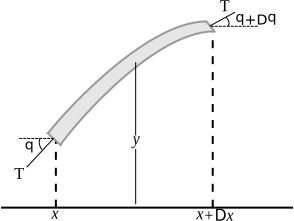
\includegraphics[height=4cm]{img/string.pdf}
\caption{Forces diagram over an element of the string with length $\Delta x$. }
\end{figure}

For a string with length $L$, linear mass density $\lambda$ and a tension $T$, let's take a small segment with small displacements in $y$. The force balance over the element showed in the Figure is:
\begin{align*}
F_y &= T \sin(\theta + \Delta \theta) - T \sin(\theta)\\
F_x &= T \cos(\theta + \Delta \theta) - T \cos(\theta) \enspace ,
\end{align*}
\end{frame}


\begin{frame}
	\frametitle{Waves in a string}
	
\begin{figure}[h]
\centering
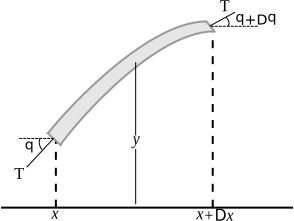
\includegraphics[height=4cm]{img/string.pdf}
\caption{Forces diagram over an element of the string with length $\Delta x$. }
\end{figure}

Taking small displacements in the string, the angles are also small and then
\begin{align*}
F_y &\approx T (\theta + \Delta \theta) - T (\theta) = T \Delta \theta\\
F_x &\approx 0 \enspace .
\end{align*}
\end{frame}


\begin{frame}
	\frametitle{Waves in a string}		
From the second Newton's law we get
\[T\ \Delta \theta = \underbrace{(\lambda\ \Delta x)}_\text{mass} a_y \enspace ,\]
if we take the limit $\Delta x \rightarrow dx$
\begin{equation}
T\ d\theta = (\lambda\ dx) a_y \enspace .
\label{eq:stringForce}
\end{equation}
And we now that $\tan \theta = \frac{\partial y}{\partial x}$, taking derivative respect $x$
\[\sec^2 \theta \frac{d\theta}{dx} = \frac{\partial^2 y}{\partial x^2} \enspace .\]
Due to small displacements $\sec^2 \theta \approx 1$, hence
\begin{equation}
d\theta \approx \frac{\partial^2 y}{\partial x^2} dx
\label{eq:stringDtheta}
\end{equation}
and replacing (\ref{eq:stringDtheta}) in  (\ref{eq:stringForce})
\[T \frac{\partial^2 y}{\partial x^2} dx = (\lambda\ dx) \frac{\partial^2 y}{\partial t^2} \enspace ,\]
we finally get the 1D Wave Equation
\[\frac{\partial^2 y}{\partial x^2} = \frac{\lambda}{T} \frac{\partial^2 y}{\partial t^2} \enspace .\]

$T/\lambda$ have square speed units, and is the square propagation speed
\[v = \sqrt{\frac{T}{\lambda}} \enspace ,\]
so
\[\frac{\partial^2 y}{\partial x^2} = \frac{1}{v^2} \frac{\partial^2 y}{\partial t^2} \enspace .\]

\end{frame}

%%% 


\end{document}

